\documentclass[thesis]{thesis-gwu}

% this package is only used to generate some random text. 
% it is not needed in a true document
\usepackage{lipsum}

\graphicspath{{../../Fig/}}

% !TEX root = ../thesis-sample.tex

% --------- FRONT MATTER PAGES ---------------------
% Title of the thesis
\title{Multi-Robot Probabilistic Mapping and Exploration}

% Author name
\author{Evan Kaufman}

% Previous degrees
\bsdepartment{Mechanical Engineering}
\bsschool{Bucknell University}
\bsgrad{May 2012}

\hidemsdegree


\showcommitteepage % hide this page if you're doing a MS thesis
%\hidecommitteepage 
\committee{ %

\vspace*{0.05\textwidth}
Taeyoung Lee, Associate Professor of Mechanical and Aerospace Engineering, Dissertation Director\\ 

James Hahn, Professor of Computer Science, Committee Member\\

Robert Pless, Professor of Computer Science, Committee Member\\

Chung Hyuk Park, Assistant Professor of Biomedical Engineering, Committee Member\\

Zhuming Ai, Computer Engineer, U.S. Naval Research Laboratory, Committee Member

}

% Chair must be entered separately for formatting reasons.
\chair{Tayeoung Lee}
\chairtitle{Associate Professor of Mechanical and Aerospace Engineering}
% Department
\department{Mechanical and Aerospace Engineering}

\phdgrad{August 31, 2018}
\defensedate{July 13, 2018}
% Year of completion for copyright page and perhaps other places
\year=2018

% Copyright page
%\copyrightholder{Someone else}

%% Dedication
%\dedication{ 
%Add here...
%%
%%This dissertation is dedicated to my parents, Elizabeth Kaufman and Stephen Kaufman, who have consistently supported me throughout my many years of education. And others...
%}

% Acknowledgments
\acknowledgments{
My academic career has certainly been a long and bumpy road, but I was never alone. I would like thank many people for their support throughout my life for pursuing difficult and interesting work.

First and foremost, I would like to thank my parents. When I was younger, I was not always a great student, but my parents believed in me. When I struggled, they helped every time. I figured that this is what all parents do, but later I realized how lucky I was. Looking back, my academic career not ending prematurely is largely thanks to my mother and father. They have loved me and supported my academic pursuits, and I am extremely grateful.

I would also like to thank all other parts of my family, including my fianc\'ee, brother, grandparents, aunts, uncles, cousins, and close friends. We make it a priority to come together and support each other, even when our careers differ greatly and our lives change unpredictably. Despite the long academic road, they provided consistent support and love.

Finally, I would like to thank my research advisor, Taeyoung Lee, for the excellent guidance over the last six years. Unlike many relationships between advisors and students, he has treated his students like colleagues rather than subordinates. This way, I could focus on completing my research objectives properly rather than trying to impress superior figure. Taeyoung Lee knew just what to say to push my research forward, even when my mind was going another direction. His positive influence over my research has been unparalleled, and I will continue using his valuable lessons.% in the years to come.

 I think that finding and pursuing a passion is something truly special. Even though I find great satisfaction in doing anything well, regardless of how simple or complicated the task, I find myself extremely fortunate to pursue endeavors that I actually find exciting and stimulating. With tremendous support around me, I begin a career in an amazing field and ready to take on future challenges.
}

% -----------------------------------------------------------------
% Typically only one of Preface/Foreward/Prologue would be in your thesis.
% To choose one simply delete the others and they will automatically dissappear

%% Preface
%\preface{
%Add here...
%%    This is the preface. 
%%    It's another front matter page that offers additional detail into your work.
%%    Typically, only one (preface OR prologue OR foreword) is used. 
%%    You can remove the other sections by deleting them inside \texttt{tex/frontmatter.tex} or using the appropriate show or hide commands.
%}

%\prologue{
%    This is the prologue. 
%    It's another front matter page that offers additional detail into your work.
%    Typically, only one (preface OR prologue OR foreword) is used. 
%    You can remove the other sections by deleting them inside \texttt{tex/frontmatter.tex} or using the appropriate show or hide commands.
%}
%
%\foreword[2]{
%    This is the foreword. 
%    It's another front matter page that offers additional detail into your work.
%    Typically, only one (preface OR prologue OR foreword) is used. 
%    You can remove the other sections by deleting them inside \texttt{tex/frontmatter.tex} or using the appropriate show or hide commands.
%}
% ----------------------------------------------------------------------

% commands to show or hide front matter pages

\showcopyright
\showabstract
\showcommitteepage
\hidededication
\showacknowledgments
\hidepreface
\hideprologue
\hideforeword

% ------------ TABLE OF CONTENTS ----------------------
% Commands to hide or show lists of figures, tables, etc.
\showlistoffigures
\hidelistoftables
\hidenomenclature

% --------- ACRONYMS and SYMBOLS ------------------------------
% TODO Deprecate the entire acronym package and switch to glossaries

% You can either use the acronymn or glossaries package (both work)
% Definition of any abbreviations used.
\abbreviations{
    \acro{CRTBP}{Circular Restricted Three Body Problem}
    \acro{NSA}{National Security Agency}
    \acro{SSME}{Space Shuttle Main Engine}
}
% call an abbreviation using \ac{abbrev}

% symbols and acronyms only show up when used in the text
\symbols{
    \acro{J}{Moment of Inertia}
}       

% if you want acronymn (simpler) then change these to show
\hidelistofabbreviations
\hidelistofsymbols

% if you want glossaries (more powerful) then leave above as hide
% GLOSSARIES package options - automatically turns off front pages from acronym package

% acronymns and symbols are basically the same, but there are two provided 
% locations where they can show up
\setabbreviationstyle[acronym]{long-short}
\setabbreviationstyle[abbreviation]{long-short}
\makeglossaries
% you can hide/show the glossaries page
\hideglossarieslistofabbreviations
\hideglossarieslistofsymbols
\hideglossariesglossaryofterms

\abstract{
This dissertation focuses on robotic mapping and exploration of uncertain environments. Computational algorithms are developed to provide complete stochastic information of the environments. These algorithms are designed for real-time implementation for robotic autonomy.

First, probabilistic occupancy grid mapping is developed according to Bayesian framework. A novel approach to this problem is explored, which uses important physical properties of the environment and stochastic properties of depth sensors. We develop an exact solution to occupancy grid probability that can be achieved in real-time using sensor properties and conventional assumptions of an occupancy grid. The rapid computation allows the algorithm to consider large scans of measurements in 2D and 3D environments. The mapping algorithm is demonstrated with several numerical examples and experiments.

The next topic is autonomous exploration, where a robot selects actions to maximize its knowledge about the probabilistic map. We select Shannon's entropy as a metric that represents grid cell uncertainty. Using the earlier contributions on probabilistic occupancy grid mapping, we determine the expected value of entropy change from possible future measurements. This entropy change provides important insights for where a robot should move to maximize its mapping information gain. Dijkstra's search is integral to the algorithm to account for collision-free distances during motion planning. This algorithm is designed for 2D and 3D, where computation time is carefully considered to ensure real-time algorithm performance. Several versions of the exploration algorithm are applied to simulations and experiments.

The final topic of this dissertation relates to multi-vehicle cooperative scenarios. The mapping algorithm is revised to accept measurements from multiple sources with differing sensor properties. More importantly, the exploration algorithm structure is modified with a bidding-based framework. A series of auctions determines where robots should travel such that the members act together as a team. This solution is further extended to multi-vehicle patrol, where robots begin with an uncertain map, autonomously explore the space, and periodically revisit regions. Autonomous multi-vehicle patrol is accomplished through map degradation, where the probabilistic map becomes more uncertain over time, and the robots must revisit these spaces. These complex algorithms are demonstrated with numerical simulations.

In short, this dissertation proposes novel solutions to probabilistic occupancy grid mapping, autonomous exploration, and patrol in single-vehicle and multi-vehicle scenarios. Real-time implementation is paramount to ensure autonomy during a task. The efficacy of the approaches are shown with several experiments and numerical examples. 

}









%% DOCUMENT AREA
\begin{document}

%% !TEX root = ../thesis-sample.tex

\chapter{Probabilistic Occupancy Grid Mapping} \label{chap:pogm}

% Add here

\section{Inverse Sensor Model}

\subsection{Bayesian Probability}

\subsection{Computationally-Efficient Solution}
% Include Fig 1 from JINT 2017

\section{Multi-Dimensional Maps}

\subsection{Ray Casting}

\subsection{Combining Measurements from a Single Scan}

\paragraph{Ray-By-Ray Approach}

\paragraph{Synergistic Update Approach}

\subsection{Multi-Sensor Fusion}

\subsection{Practical Implications}

\section{Numerical and Experimental Examples}

\subsection{Mapping a Room}
% ACC16 comparison of exact/approx. inverse sensor models

\subsection{Kinect Measurement Scan Analysis}
% ACC16 Single scan exact/approx. comparison


\section{Conclusions}




\chapter{Introduction} \label{chap:intro}

This dissertation explores three key aspects of mobile robotics: occupancy grid mapping, autonomous exploration, and cooperation among robot teams. Several novel contributions are presented on both related topics for complex and dynamic situations.


\section{Motivation and Goals}

The study of robotics has expanded tremendously in recent years as robots have taken on dangerous, difficult, and repetitive tasks instead of humans. Certain tasks, such as search-and-rescue, surveillance, and cleaning, require some level of autonomy, particularly with mobile robots exploring new and uncertain environments. While these tasks provide significant value to our society, they present nontrivial challenges for the robots, particularly in mapping, exploration, and cooperation.


\subsection{Building Probabilistic Maps}

The first topic this dissertation addresses is building accurate probabilistic maps, known as \emph{mapping}. Map generation is crucial for simultaneous localization and mapping (SLAM) because maps provide important information for the robot to determine its pose (localization), which includes its position and attitude. Mapping also provides knowledge for trajectory planning through an environment and collision avoidance with mapped obstacles. In short, mapping is of fundamental importance in mobile robotics.

Therefore, mapping quality deserves much attention. Robotics is inherently \emph{probabilistic}; no sensor reading or action from an actuator is deterministic. All robotic processes have some degree of uncertainty, and the mapping must account for this. Onboard sensors serve to improve the understanding of surrounding spaces, but the stochastic properties of those sensors must be reflected in the stochastic properties of the map. Therefore, we propose to develop probabilistic map that accounts for the history of measurements and poses, and their associated stochastic properties. Here, each element of the map holds a probability based on measured data. In turn, this probability can be applied to tasks such as collision-avoidance and predicting future map outcomes.


\subsection{Exploration in Uncertain Spaces}

The second topic of this dissertation focusses on the motions robots must choose to maximize their knowledge about the map while avoiding collisions, known as \emph{autonomous exploration}.

\subsection{Cooperation Among Autonomous Systems}

The final topic of this dissertation is cooperation among members of a robot team.

\section{Literature Review}

In this section, we discuss the existing approaches to occupancy grid mapping, autonomous exploration, and multi-vehicle cooperation. Several shortcomings with existing approaches are highlighted, which are addressed in the dissertation contributions.

\subsection{Occupancy Grid Mapping}

Here we describe the existing approaches to building probabilistic occupancy grid maps. Though several variations have been proposed, no approach uses the stochastic properties of depth sensors directly to obtain an exact Bayesian solution that can be computed in real-time.

\paragraph{Inverse Sensor Model} The key to generating a probabilistic occupancy grid map is known as the \emph{inverse sensor model}~\cite{ThrBurFox05}. The main idea is that a depth sensor has a probability density (e.g. Gaussian) that describes the stochastic properties of a sensor reading (e.g. a LIDAR range) with respect to the expected value of a reading (e.g. distance to a wall). This probability density is referred to as the \emph{forward sensor model}, as it relates a depth measurement conditioned on the occupancy of the map. 

In contrast, the inverse sensor model relates the occupancy of the map conditioned on the depth measurement. This problem is solved using Bayes' theorem. However, the occupancy grid map properties yield a complicated Bayesian probability; the computational cost has exponential complexity with respect to the number of grid cells captured within the depth sensor limits. It was previously-believed that this restriction makes solving the inverse sensor model in real-time impossible. This motivated approximate or estimated solutions, described next.

\paragraph{Approximated Function for the Inverse Sensor Model} Moravec and Elfes originally proposed a grid cell-based mapping for sonar sensors in~\cite{MorElf85}, and the probabilistic properties of the occupancy grid were formalized in~\cite{MorElf85,Elf89}. This approach models measurements with Gaussian probability density, although the occupancy of grid cells is not exactly known. Instead, the probability of grid cells are estimated with a Gaussian-like \emph{approximate function}. The authors show that occupancy probability converges to a final value following a Bayesian framework, though there is no conclusive proof that this probability is accurate. Nevertheless, this approach garnered much attention because it could efficiently produce robotic maps that nicely-resembled the occupancy of spaces around a robot.

Several other research studies have applied approximate functions in place of the inverse sensor model. For example, \cite{ChoLynHutKanBurKavThr05} proposed a simplified continuous function composed of lines patched together near a measurement reading. Furthermore, variations of approximate smoother functions in~\cite{and09,PirRutBisSch11,KhoElb12} contain Gaussian-like terms to apply occupancy grid mapping to 3D environments with more modern sensors. Numerous research studies have used the proposed approximate functions with questionable accuracy.

\paragraph{Learning the Inverse Sensor Model} The approximate nature of the inverse sensor model motivated a solution using machine learning. The main idea is to simulate maps, robot poses, and measurements with simulated noised based on the sensor stochastic properties. Then, an approximation the inverse sensor model is learned using an expectation maximization algorithm~\cite{Thr01,ThrBurFox05}. Unlike approximate functions based on intuition, the machine learning approach is based on the physical properties of sensors. However, this approach is undesirable in practice due to complexities associated to implementing a learning algorithm. For example, the accuracy of such inverse sensor models strongly depends on the samples selected for learning, but it is unclear how to select those samples, or how many samples are required to obtain a reasonable approximation. Furthermore, it is challenging to apply any learning algorithm over the large dimensional space composed of maps, poses, and measurements.

\paragraph{Log-Odds Ratio} Both approaches described above use the log-odds ratio to update grid cell probabilities. The log-odds ratio formulation is a popular framework for updating binary random variables with static state within a Bayesian filter. The main idea is that instead of multiplying terms from prior and current time steps, the properties of logarithms allow these terms to be simply added, while avoiding some truncation issues associated with probabilities close to $0$ or $1$~\cite{ThrBurFox05}. This approach is also popular because the inverse sensor model needs not consider prior probabilities. Instead, these approaches typically consider fixed uniform initial probabilities of all grid cells, which makes the formulation simpler.

However, the log-odds ratio formulation makes an assumption that is not consistent with the occupancy grid mapping problem. The approach yields a simplified solution by assuming that the probability of a measurement is independent of past measurements and robot poses. This assumption is frequently violated when past measurements and poses indicate the occupancy of other cells between the robot and the cell in question. As such, this approach neglects potentially important information when considering grid cell occupancy probability.

In short, other existing solutions to occupancy probability are inexact, and involve a potentially-harmful log-odds ratio assumption. These shortcomings motivate an exact solution to occupancy grid mapping that can be computed in real-time.

%It was previously-believed that the exact solution to occupancy grid mapping was impossible in real-time.



\subsection{Autonomous Exploration}

The next topic this dissertation addresses is autonomous exploration. The vast majority of work in simultaneous localization and mapping (SLAM) deals only with the aspect of estimating the environment and the poses of vehicles. These approaches are passive in the sense that SLAM is performed on incoming sensor measurements from vehicles following an arbitrary path. As such, human teleoperation and monitoring are often essential to guide the vehicles safely through unknown surroundings. Therefore, it is desirable that an active motion planning scheme is developed and integrated with SLAM such that vehicles are able to determine their path without human intervention, and explore unknown areas autonomously. The two approaches used to solve this problem are described next.

\paragraph{Frontier-Based Autonomous Exploration}

The most popular approach to solve the autonomous exploration problem is known as frontier-based exploration, originally-proposed in~\cite{Yam97,Yam98} for 2D applications, and was later extended to 3D with a visibility metric in~\cite{SawKriSri09} and~\cite{ZhuDinLinWu15,SenWan16,KleDor13} using the popular Octomap representation (a variation on occupancy grid mapping). The main idea is that robots toward the border between certain and uncertain space, referred to as a frontier. Then the robot takes depth measurement at this frontier, thus pushing back the boundary. This process is repeated until the map is well-known. Frontier-based exploration assumes that repeatedly moving toward the closest frontier and taking measurements are the best actions to gain new information about the map. However, these systematic actions, based on ad-hoc rules for what constitutes a frontier, do not consider the future uncertainty of the probabilistic map. Frontier-based approaches provide an intuitive solution, but lack optimality in map uncertainty or exploration time.

\paragraph{Entropy-Based Autonomous Exploration}
Entropy-based approaches address the suboptimal nature of frontier-based approaches by selecting robotic actions designed to decrease minimize map uncertainty~\cite{StaGriBur05,BurMooStaSch05}. These approaches use a measure of uncertainty known as Shannon's entropy, which becomes smaller as cell probabilities approach $0$ or $1$ (becoming more certain). Existing entropy-based approaches simulate possible future measurements from various locations with so-called ``hallucination measurements,'' which typically corresponds to expected depth measurements from the robot to the closest grid cell that is possibly occupied. Then, the robot analyzes how this measurement would affect the map uncertainty. However, this approach assumes that expected map entropy is equivalent to map entropy from expected measurements. This is not the case in general, however, as there is typically a nonzero probability that the hallucination measurement and true future measurement are not the same. Entropy-based approaches seek to optimize map uncertainty, but require large approximations which can decrease the accuracy of predictions.

In conclusion, existing autonomous exploration approaches are effective for eliminating the need for humans to control the robot. However, optimality remains quite difficult, so these approaches apply suboptimal or approximated solutions to achieve autonomous motions.


\subsection{Multi-Vehicle Cooperation}

The final topic relates to coordinating robotic efforts to build occupancy grid maps together. These concepts are further extended to autonomous cooperative patrol, where robots periodically revisit regions to monitor a large environment.

\paragraph{Cooperative Autonomous Exploration}



\paragraph{Autonomous Patrol}



\

In short, ...

\section{Outline of Dissertation}

ADD ONCE COMPLETE

\section{Contributions}

There are three key contributions in this dissertation. The first two are novel solutions that find exact occupancy probabilities and predicted entropies, respectively. These contributions improve the quality and efficiency of autonomous mapping and exploration of uncertain environments for single-vehicle missions. The third contribution extends these concepts to multi-vehicle scenarios, where multiple members of a team work together to autonomously explore and patrol large environments.




\subsection{Summary of Contributions}

The first contribution is an exact Bayesian solution to occupancy grid mapping. The proposed approach considers that occupied spaces occlude measurement behind them, which allows certain mapping outcomes to be systematically grouped together. The exact solution to occupancy grid cell probability, which was previously-believed to have exponential complexity, is now possible to solve in real-time. Numerous numerical simulations and experiments demonstrate that the proposed mapping approach is effective and inexpensive in 2D and 3D scenarios.

% JINT17: This paper proposes a computationally efficient algo- rithm to construct the exact inverse sensor model. More explicitly, for a given forward sensor model defined by the probability distribution of range measurements, this algo- rithm yields the a posteriori probabilities of occupancy of all the cells within the area covered by the range sensor from the range measurements. The key idea is reducing the computational load by using the fact that if a cell is occu- pied, the occupancies of the other cells blocked by it is irrelevant to the forward sensor model, and this property is systematically utilized with various probabilistic prop- erties to derive a computationally-efficient solution to the inverse sensor model. Furthermore, the proposed approach integrates a priori probabilities of occupancy and multiple range measurements according to the Bayesian framework to obtain more accurate maps. As such, it contrasts from the existing framework based on log-odds ratios that impose an additional Markov assumption.


The second contribution is a new approach to autonomous exploration, where the robot predicts future occupancy grid map uncertainty, using a measure known as Shannon's entropy. This approach computes the expected values of grid cell entropies from potential future measurement rays with a novel approach to predict future measurement probabilities. These predictions are used to evaluate the benefit of possible robot actions to maximize map information gain. Then, we formulate autonomous exploration as an optimization problem to maximize an objective function that includes map uncertainty and travel costs. The probabilistic map is used for collision-avoidance and motion planning. These processes are designed for real-time applications, where the robot makes decisions as it learns information about the surrounding environment.

The final contribution coordinates the mapping and exploration efforts of multiple robots together. The mapping process is multi-threaded such that multiple members update the same occupancy grid. The exploration algorithm follows a bidding-based structure. Robots compete for tasks in a series of auctions, where the winning bid of one auction affects the bids of subsequent auctions, thereby coordinating the robot efforts. This cooperative approach is computationally-efficient in large environments, and follows a receding-horizon framework, such that map expected information gains are updated as quickly as possible. The proposed coordination is extended to autonomous patrol, where occupancy grid map probabilities are degraded over time, which promotes the robots to revisit areas periodically.

\subsection{List of Publications}

The following is a list of publications. These include research included in this dissertation, as well as contributions in control, data association, and estimation.

% TODO: update this list

\begin{itemize}
	\item E. Kaufman, K. Takami, T. Lee, and Z. Ai, ``Autonomous Exploration with Exact Inverse Sensor Models,'' \textit{Journal of Intelligent }\&\textit{ Robotic Systems}, 2016, submitted.
	\item E. Kaufman, T. Lee, and Z. Ai, ``Autonomous Exploration by Expected Information Gain from Probabilistic Occupancy Grid Mapping,'' \textit{IEEE International Conference on Simulation, Modeling, and Programming for Autonomous Robots}, San Francisco, December 2016, accepted.
	\item E. Kaufman, T. Lee, Z. Ai, and I. S. Moskowitz, ``Bayesian Occupancy Grid Mapping via an Exact Inverse Sensor Model,'' \textit{Proceedings of the American Control Conference}, Boston, July 2016, pp. 5709-5715.
	\item E. Kaufman, T. A. Lovell, and T. Lee, ``Nonlinear Observability Measure for Relative Orbit Determination with Angles-Only Measurements,'' \textit{The Journal of the Astronautical Sciences}, 63(1): pp. 60-80, 2016, doi: 10.1007/s40295-015-0082-9.
	\item E. Kaufman, T. A. Lovell, and T. Lee, ``Minimum Uncertainty JPDA Filters and Coalescence Avoidance for Multiple Object Tracking,'' \textit{The Journal of the Astronautical Sciences}, 63(4): pp. 308-334, 2016, doi: 10.1007/s40295-016-0092-2.
	\item T. Wu, E. Kaufman, and T. Lee, ``Globally Asymptotically Stable Attitude Observer on SO(3),'' \textit{Proceedings of the 54th IEEE Conference on Decision and Control}, pp. 2164-2168, Osaka, Japan, December 2015.
	\item E. Kaufman, T. A. Lovell, and T. Lee, ``Nonlinear Observability Measure for Relative Orbit Determination with Angles-Only Measurements,'' \textit{Proceedings of the 25th AAS/AIAA Space Flight Mechanics Meeting}, Williamsburg, VA, Jan. 2015, AAS 15-451.
	\item E. Kaufman, T. A. Lovell, and T. Lee, ``Minimum Uncertainty JPDA Filter and Coalescence Avoidance Performance Evaluations,'' \textit{Proceedings of the 25th AAS/AIAA Space Flight Mechanics Meeting, Williamsburg}, VA, Jan. 2015, AAS 15-432.
	\item E. Kaufman, K. Caldwell, D. Lee, and T. Lee, ``Design and Development of a Free-Floating Hexrotor UAV for 6-DOF Maneuvers,'' \textit{Proceedings of the IEEE Aerospace Conference}, Mar. 2014, ASC 14-2527.
	\item E. Kaufman, T. A. Lovell, and T. Lee, ``Optimal Joint Probabilistic Data Association Filter Avoiding Coalescence in Close Proximity,'' \textit{Proceedings of the European Control Conference}, pp. 2709-2714, June 2014.
	\vspace*{0.5cm}
\end{itemize}




% !TEX root = ../thesis-sample.tex

\chapter{Probabilistic Occupancy Grid Mapping} \label{chap:pogm}

In this chapter, we present the exact solution to occupancy grid map probability. The Bayesian approach uses the stochastic properties of sensors, and exploits important patterns in conditional probabilities. This solution is simulated in several examples to show the efficacy of the approach.

\section{Mapping Problem Definition}


\section{Inverse Sensor Model}

\subsection{Bayesian Probability}

\subsection{Computationally-Efficient Solution}
% Include Fig 1 from JINT 2017

\section{Multi-Dimensional Maps}

\subsection{Ray Casting}

\subsection{Combining Measurements from a Single Scan}

Next, we describe two approaches to combine the solutions to the inverse sensor model for a single measurement ray...

\paragraph{Ray-By-Ray Approach}

\paragraph{Synergistic Update Approach}

\subsection{Multi-Sensor Fusion}

\subsection{Practical Implications}

\section{Numerical and Experimental Examples}

\subsection{Mapping a Room}
% ACC16 comparison of exact/approx. inverse sensor models

\subsection{Kinect Measurement Scan Analysis}
% ACC16 Single scan exact/approx. comparison


\section{Conclusions}


% !TEX root = ../thesis-sample.tex

\chapter{Autonomous Exploration in 2D Space} \label{chap:ae2D}

The goal of autonomous exploration is to select robotic actions designed to minimize map uncertainty, thereby maximizing map information gain. We formulate autonomous exploration as an optimization problem to determine a policy that accounts for map uncertainty and travel cost.

\section{Entropy-Based Exploration}

In this section, we define Shannon's entropy as a measure of map uncertainty, and present a novel approach to predict future entropy from an arbitrary ray. Then we discuss computational modifications for real-time implementation.

\subsection{Shannon's Entropy}

Here we present how the probabilistic properties of an occupancy grid map provide key information about the uncertainty of the space for motion planning. Shannon's entropy commonly serves as an uncertainty measure~\cite{StaGriBur05}. Provided grid cell probabilities of map $m$, Shannon's entropy is defined as
\begin{align}
\label{eqn:ShannonsEntropyCell}
H(P(\mathbf{m}_i))&=-P(\mathbf{m}_i)\log{P(\mathbf{m}_i})-P(\bar{\mathbf{m}}_i)\log{P(\bar{\mathbf{m}}_i}),
\\
\label{eqn:ShannonsEntropyMap}
H(P(m))&=\sum_{i=1}^{n_m}H(P(\mathbf{m}_i)),
\end{align}
for an individual cell and the entire map, respectively.
Thus, entropy is maximized when $P(\mathbf{m}_i)=0.5$, which corresponds to the largest uncertainty; similarly, entropy is minimized as $P(\mathbf{m}_i)$ approaches $0$ or $1$, which corresponds to the smallest uncertainty. %; thus Shannon's entropy is a measure of uncertainty.



\subsection{Expected Information Gain}

Suppose a future pose candidate and its associated future measurement scan is $X_c=\braces{x_c,R_c}$ and $Z_c$, respectively, where $c\in\mathcal C$ such that $\mathcal C=\braces{1,2,...,n_c}$ accounts for all $n_c$ candidates under consideration for the next robot pose. The current pose of the robot is \emph{not} $X_c$ in general, so any change to the probabilistic map from $X_c$ must be predicted. Much like the probabilistic mapping, this is achieved ray-by-ray~\cite{KauAiLee16,KauTakAiLee17}. Considering that all grid cell probabilities are conditioned on the history of poses $X_{1:t}$ and measurement scans $Z_{1:t}$, these terms are removed from the remaining equations for simplicity. 

\begin{prop}
\label{prop:ExpectedH}
For candidate ray $z_c$, the expected entropy is
\begin{align}
\label{eqn:DiscExpEntropyRay}
&\text{E}[H(P(m|x_c,z_{c}))]=\sum_{k=1}^{n_{r}+1}\bigg\{H(P(m|x_c,z_{c,k}))P(z_{c,k}|x_c)\bigg\},
\end{align}
where $z_{c,k}$ refers to the distance from $x_c$ to the $k$-th grid cell along the measurement ray. The first term of the summation of \refeqn{DiscExpEntropyRay}, namely $H(P(m|x_c,z_{c,k}))$, is obtained with entropy definitions \refeqn{ShannonsEntropyCell}, \refeqn{ShannonsEntropyMap} and the inverse sensor model \refeqn{RayISMAnswer}--\refeqn{Unnormalized}. The second term is derived from \refeqn{allEta} with
\begin{align}
\label{eqn:ProbMeas}
P(z_{c,k}|x_c)&=\frac{p(z_{c,k}|x_c)}{\sum_{i=1}^{n_{r}+1}p(z_{c,i}|x_c)}=\frac{\eta_{c,k}^{-1}}{\sum_{i=1}^{n_{r}+1}\eta_{c,i}^{-1}},
\end{align}
where $\eta_{c,k}$ refers to the normalizer based on the measurement $z_{c,k}$.
The expected negative entropy change for candidate pose $X_c$ is equivalently the expected information gain,
\begin{align}
\label{eqn:expectedInfoGainRay}
\mathcal I(X_c)&=H(P(m))-\text{E}\left[H(P(m|X_c,Z_c))\right].
\end{align}
\end{prop}
\begin{proof}% TODO: add ref?
See Appendix B.
\end{proof}

The proposed approach discretizes the measurement according to assumptions of occupancy grid mapping, and exploits the probabilistic properties uncovered by the proposed inverse sensor model. These are used to directly calculate the expected value of map entropy for a single measurement ray.








\subsection{Computational Limitations and Approximations}
% SIMPAR figure on entropy/computation time relationship

\section{Future Pose Optimization}

\subsection{Optimal Attitude from Sample Rays}
% SIMPAR figure on optimal pose

%Then, \refeqn{DiscExpEntropyRay} is applied repeatedly over several sample measurement rays that compose scan $Z_c$ as shown in~\cite{KauAiLee16}.

\subsection{Travel Cost with Obstacles}
% Dijkstra's cost map

\subsection{Optimal Pose Selection}
% Single-Vehicle argmax

\subsection{Collision-Free Motion Planning}
% Dijkstra's algorithm (after cost map), no least squares yet

\section{Numerical Examples}

\subsection{Exploring a Simple Environment}
% SIMPAR numerical example (2 rooms, 1 hallway)

\subsection{Exploring a Complicated Benchmark Environment}
% JINT17 Fig. 7 & 8

\section{Experimental Result}
% JINT17 9, 10, 11 (ground experiment at the NRL)

\section{Conclusions}



% !TEX root = ../thesis-sample.tex

\chapter{Autonomous Exploration in Vertically-Uniform 3D Space} \label{chap:ae3Dsimple}

\section{Occupancy Grid Mapping in 3D}

\section{Exploration in Simple Environments }

\subsection{Map Projections}

\section{Exploring a Large Room}
% IRC18 result: Fig. 4, 5, 6, 7


\section{Conclusions}





% !TEX root = ../thesis-sample.tex

\chapter{Autonomous Exploration in Complex 3D Space} \label{chap:ae3Dcomplex}

This chapter extends the autonomous exploration scheme to complex 3D environments. Unlike Chapter \ref{chap:ae2D} where exploration was applied in 2D, or Chapters \ref{chap:ae3Dsimple} and \ref{chap:multivehicle} where exploration was confined to a single height in vertically-uniform environments, this chapter proposes a completely 3D exploration approach for complex environments. This proposed approach is designed for rooms with complicated features and places with changing and uncertain terrain such as Mars.

\section{Exploration in 3D}

In this section, we propose how multiple measurement rays in 3D can determine map information gain from a pose candidate. Then, we show how a collision-free trajectory is determined with a 3D Dijkstra's search. Finally, we combine 3D information gain and travel costs into a single optimization.

\subsection{Map Information Gain in 3D}

The expected entropy for an arbitrary 1D ray spanning 3D space can be calculated with \refeqn{DiscExpEntropyRay} and \refeqn{ProbMeas} in a computationally tractable manner. However, computing the expected entropy from multiple rays simultaneously has exponential complexity, and is therefore computationally intractable. Additionally, numerous rays of a single scan commonly intersect the same grid cells, making consideration of \emph{every} measurement ray unnecessary.

Instead of considering expected entropy from a complete scan, we propose a real-time solution that selects sample measurements to determine an optimal attitude at each candidate pose and the associated map information gain, similar to how the scan information gain is found in Section \ref{sec:OptimalPose2DMap}. We assume the vehicle is capable of level flight, so the third axes of the world and body are aligned (Figure \ref{fig:transforms}), so $R_c$ can be expressed as
\begin{align*}
R_c=\begin{bmatrix}
\cos\psi & -\sin\psi & 0
\\
\sin\psi & \cos\psi & 0
\\
0 & 0 & 1
\end{bmatrix}, \quad 0\leq\psi<2\pi,
\end{align*}
where $\psi$ represents the angle about the third body-fixed axis. The direction of a 3D measurement may also have a nonzero component in the vertical direction. This is achieved by rotating the sensor frame angle $\theta$ about the second sensor-fixed axis,
\begin{align*}
R_{c,\text{sensor}}=\begin{bmatrix}
\cos\theta & 0 & \sin\theta
\\
0 & 1 & 0
\\
-\sin\theta & 0 & \cos\theta
\end{bmatrix}, \quad -\frac{\pi}{2}\leq\theta\leq\frac{\pi}{2}.
\end{align*}
Combining these two rotation matrices, the measurement $z$ with depth $\norm{z}$ is expressed with respect to a frame fixed to the world as
\begin{align}
z(\psi,\theta)=\begin{bmatrix}\cos\theta\cos\psi & -\sin\psi & \cos\psi\sin\theta
\\
\cos\theta\sin\psi & \cos\psi & \sin\psi\sin\theta
\\
-\sin\theta & 0 & \cos\theta
\end{bmatrix}
\begin{bmatrix}
\norm{z} \\ 0 \\ 0
\end{bmatrix}
=
\begin{bmatrix}
\cos\theta\cos\psi
\\
\cos\theta\sin\psi
\\
-\sin\theta
\end{bmatrix}\norm{z}.
\end{align}
In short, unit vectors are acquired via Euler angles within certain sensor limits.

% trim={<left> <lower> <right> <upper>}

\begin{figure}[!t]
	\centering
	\begin{subfigure}[t]{0.3\columnwidth}
           	\centering
          	\includegraphics[trim = {21cm 5cm 20cm 5cm}, clip, height=1.0\textwidth]{mars_general.png}
        		\caption{General View}
    	\end{subfigure}
    	\begin{subfigure}[t]{0.3\columnwidth}
           	\centering
          	\includegraphics[trim = {25cm 6cm 16cm 4cm}, clip, height=1.0\textwidth]{mars_psi.png}
        		\caption{$\psi$ Rotation}
    	\end{subfigure}
	\begin{subfigure}[t]{0.3\columnwidth}
           	\centering
          	\includegraphics[trim = {23cm 4cm 17cm 6cm}, clip, height=1.0\textwidth]{mars_theta.png}
        		\caption{$\theta$ Rotation}
    	\end{subfigure}
%\includegraphics[width=2.5in]{myfigure}
% where an .eps filename suffix will be assumed under latex, 
% and a .pdf suffix will be assumed for pdflatex; or what has been declared
% via \DeclareGraphicsExtensions.
\caption{The three frames are shown with three axes (red: first axis, green: second axis, blue: third axis). The Mars frame (short and thick) is fixed to the planet. The body-fixed frame (medium thickness and length) is fixed to the camera frame (long and narrow). The rotation of $\psi$ (b) represents the fixed camera yaw rotation and $\theta$ (c) represents the downward angle of the camera to capture the surface of Mars below the flying robot.}
\label{fig:transforms}
\end{figure}


Next, we show how multiple 3D measurements provide an estimate for information gain. Let $\Psi$ and $\Theta$ be the angular ranges for the sensor FOV in the horizontal and vertical directions, respectively. Within the sensor FOV, we select sample measurements for evaluating their expected information gains. Let the number of sample measurements be $n_\psi$ and $n_\theta$ for horizontal and vertical rotations, respectively. Since $R_c$ and the FOV are known, the set of sample measurement rays, namely $\mathcal{Z}(R_c)$, is known as well. Then, the expected information gain for a single measurement ray $z$ from candidate position $x_c$ and attitude $R_c$ is the negative expected entropy change,
\begin{align}
\label{eqn:Iray}
\mathcal{I}&_\text{ray}(x_c,R_c,\psi,\theta)\nonumber\\&=
\begin{cases}
H(P(r))-\text{E}[H(P(r|x_c,z(\psi+\tilde{\psi},\theta+\tilde{\theta})))], & \mbox{if } z(\psi+\tilde{\psi},\theta+\tilde{\theta})\in\mathcal{Z}(R_c), \\ 
0,                                                                                    & \mbox{otherwise},
\end{cases}
\end{align}
where the mounting yaw $\tilde{\psi}$ and pitch $\tilde{\theta}$ of the sensor is a fixed rotation in the horizontal and vertical directions, respectively in that order, such that $-\pi<\tilde{\psi}\leq\pi$ and $-\frac{\pi}{2}+\frac\Theta2\leq\tilde{\theta}\leq\frac{\pi}{2}-\frac\Theta2$. A positive $\tilde{\theta}$ corresponds to rotating the depth sensor from a forward direction to a downward direction toward the ground below. The expected information gain for the full scan is the summation of expected information gains for individual rays
\begin{align}
\label{eqn:Iscan}
\mathcal{I}_\text{scan}(x_c,R_c)=\sum_{i_\psi=1}^{n_\psi}\sum_{i_\theta=1}^{n_\theta}\mathcal{I}_\text{ray}\left(x_c,R_c,\frac{(2i_\psi-n_\psi-1)\Psi}{2n_\psi},\frac{(2i_\theta-n_\theta-1)\Theta}{2n_\theta}\right).
\end{align}

Finally, \refeqn{Iscan} is computed for $n_\psi$ possible attitudes when the robot is at location $x_c$, one corresponding to each yaw angle $\psi$. Then, the optimal attitude at $x_c$ is
\begin{align}
\label{eqn:RcStar}
R_c^*=\argmax_{R_c} \mathcal{I}_\text{scan}(x_c,R_c).
\end{align}

In short, the expected information gain from each possible measurement ray is obtained using predicted entropy from \refeqn{DiscExpEntropyRay} and \refeqn{ProbMeas}. Then the expected information gain from all possible scans at a candidate location is calculated from \refeqn{Iray} and \refeqn{Iscan}. Finally, the optimal attitude at this candidate location is found using \refeqn{RcStar}.

\subsection{Collision-Free Trajectory in 3D}

Next, we present a fairly straightforward application of Dijkstra's search to 3D occupancy grid mapping. First we reduced the number of grid cells to cubic blocks large enough for a robot to fit completely inside. Based on the occupancy probability of these blocks and their neighbors, we determine which cells are reachable, and what are their travel costs by building a cost map based on Dijkstra's algorithm.

Here we describe how a reduced map is generated for collision avoidance and motion planning. If the largest edge-to-edge distance of the robot, namely $\rho$, is not larger than the 3D grid cell size $\alpha$, this step is unnecessary. Let $k\geq1$ be an integer such that $k\alpha\geq\rho$ and $(k-1)\alpha<\rho$, i.e., $k$ is the minimum number of grid cells in each dimension capable of fully-enclosing the robot inside this cube. Then, we decompose the complete probabilistic 3D into map $ m_\text{reduced}$, which is composed of larger cubic cells that encompass $k^3$ cells from map $ m$. Let $\mathbf{m}_{\text{reduced},k}$ denote the $k$-th cell of $ m_\text{reduced}$ being occupied, and let $a_k\subset m$ be those $k^3$ cells from $ m$ composing this larger cell. Then, we apply the same criteria as \refeqn{CombinationProjection2DMap} to obtain the probability of $\mathbf{m}_{\text{reduced},k}$ in 3D,

\begin{align}
\label{eqn:Proj3DMapComb}
P(\mathbf{m}_{\text{reduced},k})= 
\begin{cases}
    \max_{i\in a_k}{P(\mathbf{m}_i)},	&\text{if} \ \max_{i\in a_k}{P(\mathbf{m}_i)}\geq P_\text{thresh},\\
    \min_{i\in a_k}{P(\mathbf{m}_i)},	& \text{otherwise},
\end{cases}
\end{align}
where initial probability is $0<P_\text{init}<1$ and the threshold probability is constrained to $P_\text{init}<P_\text{thresh}<1$. This approach uses probabilities that have changed from $P_\text{init}$, and favors occupied cells to avoid risking collisions.

Next, we show how $\mathbf{m}_{\text{reduced},k}$ is used in Dijkstra's search for collision avoidance and motion planning. Defining $0<P_\text{coll}<1$ as the acceptable probability of collision, every grid cell of $ m_\text{reduced}$ is considered a safe and unvisited node if its occupancy probability, and the occupancy probabilities of its neighbors (sharing a face, edge, or corner), are below $P_\text{coll}$. A cost map is built from the starting robot location by neighboring nodes, where the cost to travel to another node is based on Euclidian distance: a cell sharing a face is $\alpha$ away, a cell sharing an edge is $\sqrt2\alpha$ away, and a cell sharing a corner is $\sqrt3\alpha$ away. Generating a cost map for all reachable cells in $\mathbf{m}_{\text{reduced},k}$ provides a collision-free travel cost for all reachable candidate pose locations. Once an optimal pose is selected, the path is easily found from the cost map using steepest descent.


\subsection{Optimal 3D Pose}

Here we present how an optimal pose is selected based on information gains at optimal attitudes and known collision-free travel costs. This process is similar to prior the autonomous exploration proposed in earlier chapters, with a few minor differences.

The proposed 3D autonomous exploration follows a receding-horizon framework, and uses a bump function \refeqn{BumpFunIncreasing}--\refeqn{BumpFun} to account for travel distance. The only difference is that the start of the bump function $B_1(d)=f_\text{max}$, illustrated in Figure \ref{fig:recedingHorizonBumpFun}). This change, though minor, avoids the possible scenario where a robot repeatedly alternates between neighboring candidates with similar expected information gains.
Then, we incorporate expected information gain and travel costs into a unified optimization. Given $d(x_c)$ from Dijkstra's cost map, the optimal candidate location is
\begin{align}
\label{eqn:CandidateLocationOptimization}
x_c^*=\argmax_{x_c}\mathcal{I}_\text{scan}(x_c,R_c^*)\mathcal B(d(x_c)),
\end{align}
and therefore the optimal pose is $X_c^*=\braces{x_c^*,R_c^*}$.

	\begin{figure}
	\vspace*{-0.3\columnwidth}
		\centerline{
			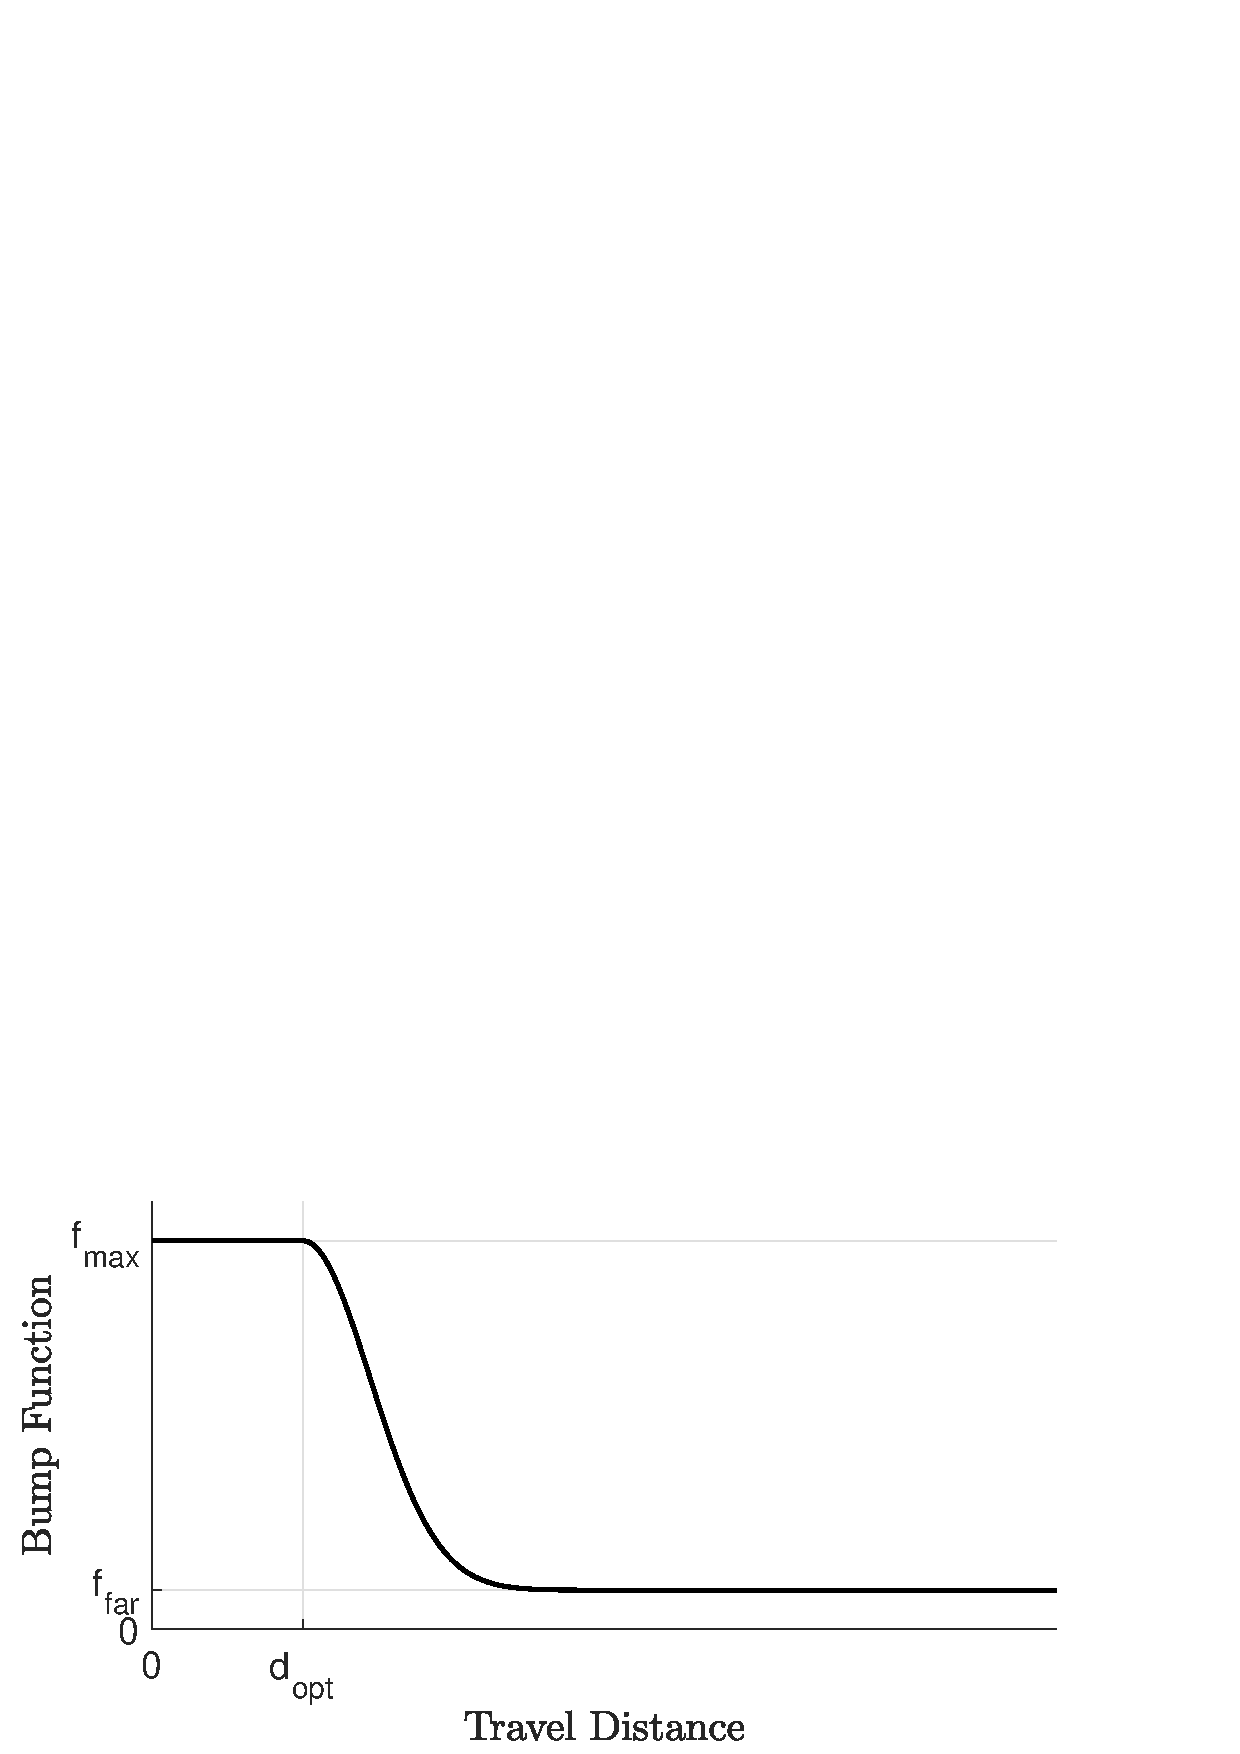
\includegraphics[width=0.6\columnwidth]{recedingHorizonBumpFunFlattened.pdf}
		}
	\vspace*{-0.25\columnwidth}
		\caption{The bump function is multiplied to the objective function of \refeqn{CandidateLocationOptimization} to prioritize local trajectories to avoid traversals across the map, where travel costs are determined using Dijkstra's algorithm. However, there is no time wasted up to $d_\text{opt}$ because this distance may be achieved in the minimum exploration computation time.}
		\label{fig:recedingHorizonBumpFun}
	\end{figure}
	
In conclusion, every reachable candidate pose is considered for its optimal attitude, which is found using sample rays spanning 3D space. The travel costs, acquired from Dijkstra's search, serve as input for the bump function, which prioritizes local trajectories to avoid costly map traversals. Then, the optimal candidate location is selected to maximize a combination of expected information gain and travel cost.



\section{Numerical Simulation}
In this section, we demonstrate the efficacy of the proposed 3D mapping and autonomous exploration with a simulated Mars environment. First we cover the parameters, then compare results using two different maps for entropy prediction.

\subsection{Mars Parameters}

A 3D environment of Mars is simulated in Gazebo. A height map~\cite{mapaplanet} is used to generate a contoured surface, and the corresponding picture of Mars is draped over this contour, shown in Figure \ref{fig:MarsGazebo}. A 3D laser scanner is also simulated in Gazebo. In the horizontal direction, the sensor has limits $\Psi=120^{\circ}$ with a total of $1000$ measurement rays inside, the sensor is fixed at angle $\tilde{\psi}=45^{\circ}$, and $n_\psi=16$ sample measurements are used. In the vertical direction, the sensor also has limits $\Theta=120^{\circ}$ with a total of $1000$ measurement rays inside, but the sensor is fixed at angle $\tilde{\theta}=30^{\circ}$, and $n_\psi=7$ sample measurements are used. These ray samples are taken from each candidate location, which are separated $1$ m apart in each of the $3$ dimensions.

% trim={<left> <lower> <right> <upper>}


\begin{figure}[!t]
	\centering
	\begin{subfigure}[t]{0.3\columnwidth}
           	\centering
          	\includegraphics[height=0.9\textwidth]{mars_heightmap.png}
        		\caption{Height Map}
    	\end{subfigure}
    	\begin{subfigure}[t]{0.3\columnwidth}
           	\centering
          	\includegraphics[height=0.9\textwidth]{mars_colormap.png}
        		\caption{Color Map}
    	\end{subfigure}
    	\begin{subfigure}[t]{0.3\columnwidth}
           	\centering{
          	\includegraphics[height=0.9\textwidth]{mars_gazebo_full_lighting.png}}
        		\caption{Gazebo Environment}
    	\end{subfigure}
\caption{The height map (a) and color map (b) are combined in the Gazebo simulator (c) to model a Mars environment. The robot captures the simulated environment to generate an occupancy grid map.}
\label{fig:MarsGazebo}
\end{figure}

The map parameters are also important to the success of the exploration. The full map has dimensions $20$ m $\times$ $20$ m $\times$ $5$ m in the Mars-fixed frame, with cell edge length $\alpha=0.075$ m. The reduced map for collision-avoidance and motion planning has cells $k=3$ times the size ($0.225$ m), so $k^3=27$ cells are considered in \refeqn{Proj3DMapComb}. The bump functions use $f_\text{max}=1.0$, $f_\text{far}=0.1$, and $\beta=0.1$ to account for travel costs with \refeqn{BumpFun}. The receding horizon optimal time $d_\text{opt}$ is based on a fixed robot velocity of $0.25$ m/sec and the computation time varies from $1.8$ sec to $2.5$ sec.

\subsection{Mars Results}

The simulation was run twice. Case 1 was as described in this paper. Case 2 was identical to Case 1, except the reduced map $ m_\text{reduced}$ is used when computing \refeqn{Iscan}. Case 2 is largely inspired by the promising experimental results covered in Section \ref{sec:QuadrotorNRL}, where a projected map based on the same criteria as \refeqn{Proj3DMapComb} proved effective for level flight. The resulting occupancy grid maps for Cases 1 and 2 are shown in Figures \ref{fig:mars3DogmCase1} and \ref{fig:mars3DogmCase2}, respectively. A video of Case 1 can be found at \href{https://youtu.be/FrBcL2UMW9w}{\WriteBlue{https://youtu.be/FrBcL2UMW9w}}, and close-up pictures from Case 2 are shown in Figure \ref{fig:marsZoomedIn}. The complete map entropies for both cases are illustrated in Figure \ref{fig:mars3Dentropy}.


\begin{figure}[!t]
	\centering
	\begin{subfigure}[t]{0.49\columnwidth}
           	\centering
          	\includegraphics[height=0.5\textwidth]{FullMarsMap30sec.jpg}
        		\caption{$30$ sec}
		\vspace*{0.025\textwidth}
    	\end{subfigure}
    	\begin{subfigure}[t]{0.49\columnwidth}
           	\centering
          	\includegraphics[height=0.5\textwidth]{FullMarsMap1min.jpg}
        		\caption{$1$ min}
		\vspace*{0.025\textwidth}
    	\end{subfigure}
	\centering
	\begin{subfigure}[t]{0.49\columnwidth}
           	\centering
          	\includegraphics[height=0.5\textwidth]{FullMarsMap2min.jpg}
        		\caption{$2$ min}
		\vspace*{0.025\textwidth}
    	\end{subfigure}
    	\begin{subfigure}[t]{0.49\columnwidth}
           	\centering
          	\includegraphics[height=0.5\textwidth]{FullMarsMap3min.jpg}
        		\caption{$3$ min}
		\vspace*{0.025\textwidth}
    	\end{subfigure}
	\centering
	\begin{subfigure}[t]{0.49\columnwidth}
           	\centering
          	\includegraphics[height=0.5\textwidth]{FullMarsMap4min.jpg}
        		\caption{$4$ min}
		\vspace*{0.025\textwidth}
    	\end{subfigure}
    	\begin{subfigure}[t]{0.49\columnwidth}
           	\centering
          	\includegraphics[height=0.5\textwidth]{FullMarsMap5min.jpg}
        		\caption{$5$ min}
		\vspace*{0.025\textwidth}
    	\end{subfigure}
	\centering
	\begin{subfigure}[t]{0.49\columnwidth}
           	\centering
          	\includegraphics[height=0.5\textwidth]{FullMarsMap10min.jpg}
        		\caption{$10$ min}
		\vspace*{0.025\textwidth}
    	\end{subfigure}
    	\begin{subfigure}[t]{0.49\columnwidth}
           	\centering
          	\includegraphics[height=0.5\textwidth]{FullMarsMap15min.jpg}
        		\caption{$15$ min}
		\vspace*{0.025\textwidth}
    	\end{subfigure}
\caption{In Case 1, the robot (red disk with arrow indicating laser direction) moves toward candidate poses (red arrows, more opaque for greater reward) based on expected entropy change of the 3D probabilistic occupancy grid map $m$ (cubes: greater opacity for greater occupancy probability) of the surface of Mars.}
\label{fig:mars3DogmCase1}
\end{figure}


\begin{figure}[!t]
	\centering
	\begin{subfigure}[t]{0.49\columnwidth}
           	\centering
          	\includegraphics[height=0.5\textwidth]{RdcdMarsMap30sec.jpg}
        		\caption{$30$ sec}
		\vspace*{0.025\textwidth}
    	\end{subfigure}
    	\begin{subfigure}[t]{0.49\columnwidth}
           	\centering
          	\includegraphics[height=0.5\textwidth]{RdcdMarsMap1min.jpg}
        		\caption{$1$ min}
		\vspace*{0.025\textwidth}
    	\end{subfigure}
	\centering
	\begin{subfigure}[t]{0.49\columnwidth}
           	\centering
          	\includegraphics[height=0.5\textwidth]{RdcdMarsMap2min.jpg}
        		\caption{$2$ min}
		\vspace*{0.025\textwidth}
    	\end{subfigure}
    	\begin{subfigure}[t]{0.49\columnwidth}
           	\centering
          	\includegraphics[height=0.5\textwidth]{RdcdMarsMap3min.jpg}
        		\caption{$3$ min}
		\vspace*{0.025\textwidth}
    	\end{subfigure}
	\centering
	\begin{subfigure}[t]{0.49\columnwidth}
           	\centering
          	\includegraphics[height=0.5\textwidth]{RdcdMarsMap4min.jpg}
        		\caption{$4$ min}
		\vspace*{0.025\textwidth}
    	\end{subfigure}
    	\begin{subfigure}[t]{0.49\columnwidth}
           	\centering
          	\includegraphics[height=0.5\textwidth]{RdcdMarsMap5min.jpg}
        		\caption{$5$ min}
		\vspace*{0.025\textwidth}
    	\end{subfigure}
	\centering
	\begin{subfigure}[t]{0.49\columnwidth}
           	\centering
          	\includegraphics[height=0.5\textwidth]{RdcdMarsMap10min.jpg}
        		\caption{$10$ min}
		\vspace*{0.025\textwidth}
    	\end{subfigure}
    	\begin{subfigure}[t]{0.49\columnwidth}
           	\centering
          	\includegraphics[height=0.5\textwidth]{RdcdMarsMap15min.jpg}
        		\caption{$15$ min}
		\vspace*{0.025\textwidth}
    	\end{subfigure}
\caption{In Case 2, the robot (red disk with arrow indicating laser direction) generates a 3D probabilistic occupancy grid map $m$ (cubes: greater opacity for greater occupancy probability), which is used to generate a reduced map $m_\text{reduced}$ based on \refeqn{Proj3DMapComb}. The robot moves toward candidate poses (red arrows, more opaque for greater reward) based on expected entropy change of $m_\text{reduced}$. Using $m_\text{reduced}$ instead of $m$ for entropy calculation leads to faster exploration of new terrain, but this leaves some grid cells missing.}
\label{fig:mars3DogmCase2}
\end{figure}

\begin{figure}[!t]
	\centering
	\begin{subfigure}[t]{0.95\columnwidth}
           	\centering
          	\includegraphics[width=0.9\textwidth]{mars_closeup.png}
        		\caption{Full Map Cells and Sensor Scan}
		\vspace*{0.025\textwidth}
    	\end{subfigure}
	\centering
	\begin{subfigure}[t]{0.95\columnwidth}
           	\centering
          	\includegraphics[width=0.9\textwidth]{scitech_reducedCells.png}
        		\caption{Full Map and Reduced Map Cells}
		\vspace*{0.025\textwidth}
    	\end{subfigure}
\caption{The close-up images from the Case 2 trial show the candidate future poses (red arrows), where greater opacity represents a larger objective function of \refeqn{CandidateLocationOptimization}. In (a), we show the 3D scan with color corresponding to the surface of Mars. In (b), we overlay the full map $m$ (colored) with the reduced map $m_\text{reduced}$ (gray) from \refeqn{Proj3DMapComb}.}
\label{fig:marsZoomedIn}
\end{figure}


	\begin{figure}
		\centerline{
			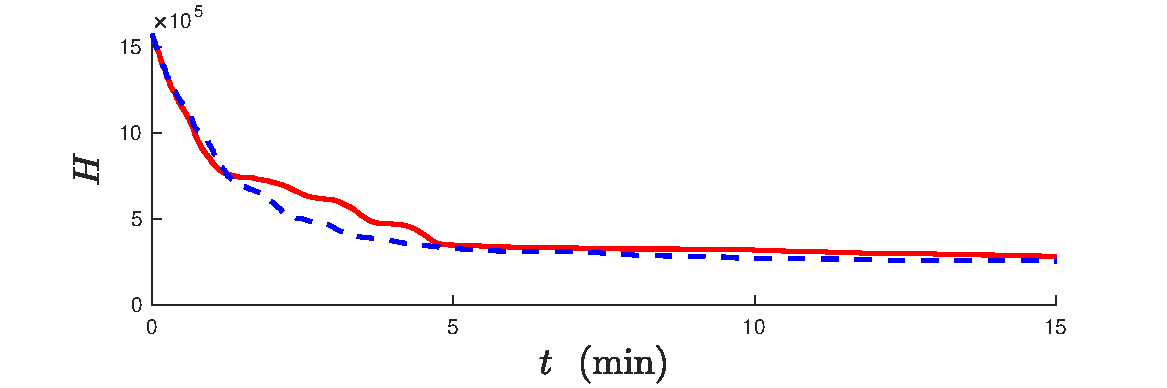
\includegraphics[width=0.6\columnwidth]{scitech_entropy_comparison_flat.pdf}
		}
		\caption{The complete map entropy for Case 1 (red solid line) decreases at roughly the same rate as the reduced map entropy for Case 2 (dashed blue line) toward the beginning. However, the expected entropy in Case 2 promotes actions toward unexplored territory, while the policy of Case 1 yields a more complete map before moving on to unexplored spaces.}
		\label{fig:mars3Dentropy}
	\end{figure}


In both cases, the robot built the 3D probabilistic map of the $2000$ cubic meter space composed of $4.74\times10^6$ grid cells. The maps were mostly complete within $10$ minutes. The $\tilde{\theta}=30^{\circ}$ downward viewing angle captured the ground nicely, as candidate attitudes tended to direct the onboard sensor toward uncertain regions on the surface of Mars. The proposed approach provided collision-free mapping and autonomous exploration in real-time.

However, the choice of occupancy grid map used for entropy predictions introduced an interesting tradeoff. In Case 1, when the full probabilistic map $m$ was used in \refeqn{Iscan}, regions where the grid cells were partially-known were frequently reconsidered until the space was well-known. Conversely in Case 2, when $m_\text{reduced}$ was used instead, the robot repeatedly left spaces that were missing a few grid cells to visit new terrain. This is because $m_\text{reduced}$ contained some cells with large occupancy probabilities based on \refeqn{Proj3DMapComb}, which allowed some grid cells of $m$ enclosed within a cell of $m_\text{reduced}$ to be uncertain. The exploration policy of Case 2 incorrectly assumed these regions were well-known. Ironically, this false assumption actually led to greater information gains when the vehicle moved on to unvisited terrain. Conversely with Case $1$, which used $m$ for computing expected entropy, the total map entropy decreased more steadily and generated a more-complete 3D occupancy grid of the surface of Mars.

In short, the proposed 3D probabilistic occupancy grid mapping and autonomous exploration were simulated successfully in real-time over the surface of Mars using ROS and Gazebo. Choosing $m$ for entropy predictions produced a more-complete map, but choosing $m_\text{reduced}$ was sometimes beneficial for exploring new terrain faster, while forgoing map completeness.



\section{Conclusions}

This chapter covers autonomous exploration through a 3D environment, such that the robot can account for complex geometries in all dimension and explore with upward and downward motions. The expected information gains are calculated with predicting the entropy changes from sample rays in 3D space, and the bump function is applied using the cost from Dijkstra's search. An example where a robot maps and explores the surface of Mars demonstrates the efficacy of the approach.




% !TEX root = ../thesis-sample.tex

\chapter{Multi-Vehicle Autonomous Exploration and Patrol} \label{chap:multivehicle}

\section{Bidding-Based Autonomous Exploration}

\subsection{Objective Function for the First Auction}

\subsection{Objective Function for Subsequent Auctions}

\subsection{Receding Horizon Framework}

\subsection{Multi-Vehicle Exploration Numerical Simulation}
% Multi-vehicle ICRA figs 3-6 (remake fig. 5 with larger contrast)

\section{Multi-Vehicle Cooperative Patrol}

\subsection{Continuous-Time Markov Process for Cell Degradation}
% JINT18 fig. 3

\subsection{Multi-Vehicle Patrol Numerical Simulation}
% JINT18 fig. 10-13 (ref. ICRA fig 3 from above in this chapter)

\section{Conclusions}







\bibliographystyle{plain}
\bibliography{../../BibSources.bib}

% appendices must appear after
% !TEX root = ../thesis-sample.tex
\appendix
\doublespacing
\chapter{Proof of Proposition 1}

\paragraph{Unnormalized Reduced Map Inverse Sensor Model}
For the reduced map of the $l$-th ray, the unnormalized probability that corresponds to the terms without $\eta_{t,l}$ in \refeqn{InvSenModWithProbDens} is given by
\begin{align}
\tilde P&(\mathbf{r}_{l,k}|z_{t,l},X_{1:t},Z_{1:t-1})= \sum_{r\in\mathcal{M}_{k}} p(z_{t,l}|r,X_t) P(r|X_{1:t-1},Z_{1:t-1}).\label{eqn:tildePlk}
\end{align}
Recall $\mathcal{M}_k$ corresponds to the set of maps where the $k$-th cell is occupied. Define a subset $\mathcal{N}_{i,k}\subset \mathcal{M}_k$ for $1\leq i\leq k$ be the set of maps where the $i$-th cell is the first occupied cell. More explicitly, 
\begin{align*}
\mathcal{N}_{i,k} & = \{ r\in\mathcal{M}_k| \mathbf{r}_{l,i+}\}= \{ r\in\mathcal{M}_k| \mathbf{r}_{l,1}=0,\ldots, \mathbf{r}_{l,i-1}=0, \mathbf{r}_{l,i}=1,
\mathbf{r}_{l,k}=1\}.
\end{align*}
Then, $\mathcal{M}_k$ can be written as $\mathcal{M}_k =\bigcup_{i=1}^{k} \mathcal{N}_{i,k}$. Using this, the summation over $\mathcal{M}_k$ at \refeqn{tildePlk} can be decomposed of the summation over each $\mathcal{N}_{i,k}$ to obtain
\begin{align*}
\tilde P(\mathbf{r}_{l,k}|z_{t,l},X_{1:t},Z_{1:t-1})= \sum_{i=1}^k\braces{\sum_{r\in\mathcal{N}_{i,k}} p(z_{t,l}|r,X_t) P(r|X_{1:t-1},Z_{1:t-1})}.
\end{align*}
This is motivated by the fact that the forward sensor model $p(z_{t,l}|r,X_t)$ is identical for all maps in $\mathcal{N}_{i,k}$, such that $p(z_{t,l}|r,X_t)=p(z_{t,l}|\mathbf{r}_{l,i+},X_t)$ and it is moved left of the summation to obtain
\begin{align}
\tilde P(\mathbf{r}_{l,k}|z_{t,l},X_{1:t},Z_{1:t-1})= \sum_{i=1}^k \braces{p(z_{t,l}|\mathbf{r}_{l,i+},X_t) \sum_{r\in\mathcal{N}_{i,k}} P(r|X_{1:t-1},Z_{1:t-1})}.\label{eqn:tildePlk0}
\end{align}
The last term of the above expression corresponds to the a priori probability of $\mathcal{N}_{i,k}$. When $i<k$, it is given by
\begin{align}
\sum_{r\in\mathcal{N}_{i,k}}  &P(r|X_{1:t-1},Z_{1:t-1}) 
\nonumber\\&= \bigg\{\prod_{j=0}^{i-1}P(\bar{\mathbf{r}}_{l,j}|X_{1:t-1},Z_{1:t-1})\bigg\}
P({\mathbf{r}}_{l,i}|X_{1:t-1},Z_{1:t-1})P({\mathbf{r}}_{l,k}|X_{1:t-1},Z_{1:t-1}),\label{eqn:PNik}
\end{align}
and when $i=k$, 
\begin{align}
\sum_{r\in\mathcal{N}_{k,k}} & P(r|X_{1:t-1},Z_{1:t-1})= \bigg\{\prod_{j=0}^{k-1}P(\bar{\mathbf{r}}_{l,j}|X_{1:t-1},Z_{1:t-1})\bigg\}P({\mathbf{r}}_{l,k}|X_{1:t-1},Z_{1:t-1}).\label{eqn:PNkk}
\end{align}
Substituting \refeqn{PNik} and \refeqn{PNkk} into \refeqn{tildePlk0}, we obtain \refeqn{Unnormalized}.



\paragraph{Complement of the Unnormalized Reduced Map Inverse Sensor Model}
An analytic expression for the complement of the unnormalized inverse sensor model is also required  for obtaining the normalizer of the $l$-th ray at time $t$, namely $\eta_{t,l}$. Let $\bar{\mathcal{M}}_k$ be the set of maps where the $k$-th cell is unoccupied, i.e., $\bar{\mathcal{M}}_k = \{ r\in\{0,1\}^{n_{r,l}}\,|\, \mathbf{r}_{l,k}=0\}$. Similar to \refeqn{tildePlk},
\begin{align}
\tilde P&(\bar{\mathbf{r}}_{l,k}|z_{t,l},X_{1:t},Z_{1:t-1})= \sum_{r\in\bar{\mathcal{M}}_{k}} p(z_{t,l}|r,X_t) P(r|X_{1:t-1},Z_{1:t-1}).\label{eqn:tildePbarlk}
\end{align}

Let $\bar{\mathcal{N}}_{i,k}\subset \bar{\mathcal{M}}_k $ for $1\leq i\leq n_{r,l}$ and $i\neq k$ be the set of maps where the $i$-th cell is the first occupied cell. More explicitly, 
\begin{align*}
\bar{\mathcal{N}}_{i,k}=\{r\in\bar{\mathcal{M}}_k\,|\, \mathbf{r}_{l,1}=0,\ldots,\mathbf{r}_{l,i-1}=0,
\mathbf{r}_{l,i}=1,\mathbf{r}_{l,k}=0\}.
\end{align*}
Then, we have $\bar{\mathcal{M}}_k=\bigcup_{\substack{i=1\\i\neq k}}^{n_{r,l}} \bar{\mathcal{N}}_{i,k}$. Note that the forward sensor model $p(z_{t,l}|r,X_t)$ is identical for any maps in $\bar{\mathcal{N}}_{i,k}$, such that $p(z_{t,l}|r,X_t)=p(z_{t,l}|\mathbf{r}_{l,i+},X_t)$. Similar to \refeqn{tildePlk0},
\begin{align}
\tilde P&(\bar{\mathbf{r}}_{l,k}|z_{t,l},X_{1:t},Z_{1:t-1})= \sum_{\substack{i=1\\i\neq k}}^{n_{r,l}} \braces{p(z_{t,l}|\mathbf{r}_{l,i+},X_t) \sum_{r\in\bar{\mathcal{N}}_{i,k}} P(r|X_{1:t-1},Z_{1:t-1})},\label{eqn:tildePbarlk0}
\end{align}
where the last term corresponds to the a priori probability of $\bar{\mathcal{N}}_{i,k}$. When $i<k$, it is given by
\begin{align}
\sum_{r\in\bar{\mathcal{N}}_{i,k}} & P(r|X_{1:t-1},Z_{1:t-1}) \nonumber\\&= \bigg\{\prod_{j=0}^{i-1}P(\bar{\mathbf{r}}_{l,j}|X_{1:t-1},Z_{1:t-1})\bigg\} P({\mathbf{r}}_{l,i}|X_{1:t-1},Z_{1:t-1})P(\bar{\mathbf{r}}_{l,k}|X_{1:t-1},Z_{1:t-1}),\label{eqn:PbarNik1}
\end{align}
and when $k<i$,
\begin{align}
\sum_{r\in\bar{\mathcal{N}}_{i,k}} & P(r|X_{1:t-1},Z_{1:t-1}) = \bigg\{\prod_{j=0}^{i-1}P(\bar{\mathbf{r}}_{l,j}|X_{1:t-1},Z_{1:t-1})\bigg\}
P({\mathbf{r}}_{l,i}|X_{1:t-1},Z_{1:t-1}).\label{eqn:PbarNik2}
\end{align}
Substituting \refeqn{PbarNik1} and \refeqn{PbarNik2} into \refeqn{tildePbarlk0}, we obtain
\begin{align}
\tilde P &(\bar{\mathbf{r}}_k|z_{t,l},X_{1:t},Z_{1:t-1})
=P(\bar{\mathbf{r}}_{l,k}|X_{1:t-1},Z_{1:t-1})\nonumber\\
&\quad\times \bigg[\sum_{i=1}^{k-1}\bigg\{\prod_{j=0}^{i-1}P(\bar{\mathbf{r}}_{l,j}|X_{1:t-1},Z_{1:t-1})\bigg\} p(z_{t,l}|\mathbf{r}_{l,i+},X_t)P(\mathbf{r}_{l,i}|X_{1:t-1},Z_{1:t-1})\bigg]
\nonumber
\\
&\quad
+
\bigg[\sum_{i=k+1}^{n_{r,l}+1}\bigg\{\prod_{j=0}^{i-1}P(\bar{\mathbf{r}}_{l,j}|X_{1:t-1},Z_{1:t-1})\bigg\} p(z_{t,l}|\mathbf{r}_{i+},X_t)P(\mathbf{r}_{l,i}|X_{1:t-1},Z_{1:t-1})\bigg],\label{eqn:tildePbar}
\end{align}
where $p(z_{t,l}|\mathbf{r}_{(n_r+1)+},X_t)$ corresponds to the forward sensor model of maximum reading and $P(\mathbf{r}_{l,n_{r,l}+1}|X_{1:t-1},Z_{1:t-1})=1$ for convenience for the empty map case.

\paragraph{Normalizer}
We have 
\begin{align*}
P(\mathbf{r}_{l,k}|z_{t,l},X_{1:t},Z_{1:t-1})+
P(\bar{\mathbf{r}}_{l,k}|z_{t,l},X_{1:t},Z_{1:t-1})=1.
\end{align*}
Since they share the same normalizer $\eta_{t,l}$, this implies 
\begin{align*}
\eta_{t,l}=[\tilde P(\mathbf{r}_{l,k}|z_{t,l},X_{1:t},Z_{1:t-1})+
\tilde P(\bar{\mathbf{r}}_{l,k}|z_{t,l},X_{1:t},Z_{1:t-1})]^{-1}.
\end{align*}
Substituting \refeqn{Unnormalized} and \refeqn{tildePbar}, and rearranging, we obtain \refeqn{allEta}.






\end{document}
